\documentclass{article}
\usepackage[utf8]{inputenc}

\documentclass[a4paper]{article}
\usepackage[12pt]{extsizes}
\usepackage{amsmath,amsthm,amssymb,float}
\usepackage[hidelinks]{hyperref} 
\renewcommand{\labelenumii}{\Roman{enumii}}
\usepackage[warn]{mathtext}
\usepackage[T1,T2A]{fontenc}
\usepackage[utf8]{inputenc}
\usepackage[english,russian]{babel}
\usepackage{tocloft}
\linespread{1.5}
\usepackage{indentfirst}
\usepackage{setspace}
%\полуторный интервал
\onehalfspacing

\newcommand{\RomanNumeralCaps}[1]
    {\MakeUppercase{\romannumeral #1}}

\usepackage{amssymb}

\usepackage{graphicx, float}
\graphicspath{{pictures/}}
\DeclareGraphicsExtensions{.pdf,.png,.jpg}
\usepackage[left=25mm,right=1cm,
    top=2cm,bottom=20mm,bindingoffset=0cm]{geometry}
\renewcommand{\cftsecleader}{\cftdotfill{\cftdotsep}}

\addto\captionsrussian{\renewcommand{\contentsname}{СОДЕРЖАНИЕ}}

\usepackage{fancyhdr}
\usepackage[nottoc]{tocbibind}

\fancypagestyle{plain}{%
\fancyhf{}
\renewcommand{\headrulewidth}{0pt}
\fancyhead[R]{\thepage}
}

\usepackage{blindtext}
\pagestyle{myheadings}
% href
\usepackage{hyperref}

\begin{document}
\begin{titlepage}
  \begin{center}
  
     
    \large
    
    Санкт-Петербургский политехнический университет Петра Великого
    
    Институт прикладной математики и механики
    
    \textbf{Высшая школа прикладной математики и вычислительной физики}
    
    \vfill
     
     
    \textsc{\textbf{\Large{Лабораторная работа №1}}}\\[5mm]
     
    {\large \textbf{Тема: <<Решение задач линейного программирования симплекс-методом>>}}
    
    \\ по дисциплине\\ <<Методы оптимизаций>>\\

\end{center}

\vfill


\begin{tabular}{l p{140} l}
Выполнили студенты \\группы 3630102/80401   

&  &Мамаева Анастасия Сергеевна\\
&  &Веденичев Дмитрий Александрович\\
&  &Тырыкин Ярослав Алексеевич\\

Руководитель\\Доцент, к.ф.-м.н.& \hspace{0pt} &   Родионова Елена Александровна \\\\
\end{tabular}

\hfill \break
\hfill \break
\begin{center} Санкт-Петербург \\2021 \end{center}
\thispagestyle{empty}
 
\end{titlepage}
\newpage
\begin{center}
    \setcounter{page}{2}
    \tableofcontents  
\end{center}

\newpage
\section{Постановка задачи}
\noindent Сформулируем задачу линейного программирования, состоящую из пяти переменных, включающую три равенства и два неравенства разных знаков. Также поставим ограничения на знаки для четырёх переменных:


\begin{equation*}
 \begin{cases}
  x_1+5x_2+3x_4+4x_5 \ge 2 
   \\
   2x_1+x_2+7x_3+2x_4+6x_5 = 3
   \\
   3x_1+3x_2+2x_3+3x_4+x_5 = 6
   \\
   8x_2+x_3+x_4+3x_5 = 2
   \\
   x_1+4x_2+4x_3+3x_4+x_5 \le 8
   \\
   x_1, x_2, x_3, x_4 \ge 0
 \end{cases}
\end{equation*}

\noindent Зададим функцию цели: $$4x_2+3x_4 \rightarrow min$$
\\
\noindent Необходимо:
\begin{enumerate} 
\item Построить к исходной задаче двойственную, затем обе задачи привести к форме, позволяющей применить к ним симплекс-метод.
\item Решить обе задачи симплекс-методом с выбором начального приближения методом искусственного базиса.
\item Исследовать влияние ошибок в коэффициентах функции цели на результат решения задачи.
\item Разработать схему восстановления прямой задачи по решению двойственной.
\item Решить данную задачу с помощью пакета MATLAB и сравнить полученные результаты.
\end{enumerate}

\section{Исследование применимости метода}
\noindent Алгоритм симплекс-метода применим для решения оптимизационных задач на поиск минимума, приведенных к канонической форме.  
\begin{equation*}
  min~c^T[N] \cdot x[N]  
\end{equation*}
\begin{equation}
S = \{\ x[N]|~ A[M, N] \cdot x[N] = b[M],~x[N] \ge 0 \}\
\label{one} 
\end{equation}

\noindent Количество строк матрицы $A$ равно $m = |M|$, а количество столбцов $n = |N|$, причем $m < n$. 
Тогда метод применим, если $rangA = m$, что будет гарантировать наличие хотя бы одного опорного вектора.\\

\noindent Проверим, выполняется ли это условие для нашей задачи.
\begin{equation*}
A =
\begin{pmatrix}
1 & 5 & 0 & 3 & 4\\
2 & 1 & 7 & 2 & 6\\
3 & 3 & 2 & 3 & 1\\
0 & 8 & 1 & 1 & 3\\
1 & 4 & 4 & 3 & 1
\end{pmatrix}
\sim
\begin{pmatrix}
1 & 5 & 0 & 3 & 4\\
0 & -9 & 7 & -4 & -2\\
0 & -12 & 2 & -6 & -11\\
0 & 8 & 1 & 1 & 3\\
0 & -1 & 4 & 0 & -3
\end{pmatrix}
\sim
\begin{pmatrix}
1 & 5 & 0 & 3 & 4\\
0 & 1 & \frac{-7}{9} & \frac{4}{9} & \frac{2}{9}\\
0 & -12 & 2 & -6 & -11\\
0 & 8 & 1 & 1 & 3\\
0 & -1 & 4 & 0 & -3
\end{pmatrix}
\sim
\end{equation*}
\begin{equation*}
\sim
  \begin{pmatrix}
1 & 5 & 0 & 3 & 4\\
0 & 1 & \frac{-7}{9} & \frac{4}{9} & \frac{2}{9}\\
0 & 0 & \frac{-22}{3} & \frac{-2}{3} & \frac{-25}{3}\\
0 & 0 & \frac{65}{9} & \frac{-23}{9} & \frac{11}{9}\\
0 & 0 & \frac{29}{9} & \frac{4}{9} & \frac{-25}{9}
\end{pmatrix} 
\sim
 \begin{pmatrix}
1 & 5 & 0 & 3 & 4\\
0 & 1 & \frac{-7}{9} & \frac{4}{9} & \frac{2}{9}\\
0 & 0 & 1 & \frac{1}{11} & \frac{25}{22}\\
0 & 0 & \frac{65}{9} & \frac{-23}{9} & \frac{11}{9}\\
0 & 0 & \frac{29}{9} & \frac{4}{9} & \frac{-25}{9}
\end{pmatrix} 
\sim
 \begin{pmatrix}
1 & 5 & 0 & 3 & 4\\
0 & 1 & \frac{-7}{9} & \frac{4}{9} & \frac{2}{9}\\
0 & 0 & 1 & \frac{1}{11} & \frac{25}{22}\\
0 & 0 & 0 & \frac{-106}{33} & \frac{-461}{66}\\
0 & 0 & 0 & \frac{5}{33} & \frac{-425}{66}
\end{pmatrix} 
\sim
\end{equation*}
\begin{equation*}
\sim
 \begin{pmatrix}
1 & 5 & 0 & 3 & 4\\
0 & 1 & \frac{-7}{9} & \frac{4}{9} & \frac{2}{9}\\
0 & 0 & 1 & \frac{1}{11} & \frac{25}{22}\\
0 & 0 & 0 & 1 & \frac{461}{212}\\
0 & 0 & 0 & \frac{5}{33} & \frac{-425}{66}
\end{pmatrix} 
\sim
\begin{pmatrix}
1 & 5 & 0 & 3 & 4\\
0 & 1 & \frac{-7}{9} & \frac{4}{9} & \frac{2}{9}\\
0 & 0 & 1 & \frac{1}{11} & \frac{25}{22}\\
0 & 0 & 0 & 1 & \frac{461}{212}\\
0 & 0 & 0 & 0 & \frac{-1435}{212}
\end{pmatrix} 
\sim
\begin{pmatrix}
1 & 5 & 0 & 3 & 4\\
0 & 1 & \frac{-7}{9} & \frac{4}{9} & \frac{2}{9}\\
0 & 0 & 1 & \frac{1}{11} & \frac{25}{22}\\
0 & 0 & 0 & 1 & \frac{461}{212}\\
0 & 0 & 0 & 0 & 1
\end{pmatrix} 
\end{equation*}
\newline
Получили пять ненулевых строк $\Rightarrow~rangA = 5$, ровно столько же, сколько строк в матрице. 

\section{Описание алгоритмов}
\subsection{Приведение задачи к канонической форме}
\label{canon}
\begin{enumerate}
    \item Если в системе есть неравенства со знаком "$\leq$"\! , то к левой части каждого из них добавляем $w_i\geq0$. В неравенствах со знаком "$\geq$"\!  из левой части вычитаем $w_i\geq0$.
    \item Полагаем все неравенства равенствами.
    \item Производим замену переменных: для $x_i\leq0$ полагаем $x^{'}_i=-x_i\geq0$. Для знакопеременных $x_i$ полагаем $x_i = u_i - v_i;\;u_i,v_i\geq0$.
\end{enumerate}

\noindent По вышеизложенному алгоритму преобразуем исходную задачу к канонической форме:

\begin{equation*}
 \begin{cases}
  x_1+5x_2+3x_4+4x_5 \ge 2 
   \\
   2x_1+x_2+7x_3+2x_4+6x_5 = 3
   \\
   3x_1+3x_2+2x_3+3x_4+x_5 = 6
   \\
   8x_2+x_3+x_4+3x_5 = 2
   \\
   x_1+4x_2+4x_3+3x_4+x_5 \le 8
   \\
   x_1, x_2, x_3, x_4 \ge 0
 \end{cases}
 \Rightarrow
 \begin{cases}
  x_1+5x_2+3x_4+4x_5-x_6 = 2 
   \\
   2x_1+x_2+7x_3+2x_4+6x_5 = 3
   \\
   3x_1+3x_2+2x_3+3x_4+x_5 = 6
   \\
   8x_2+x_3+x_4+3x_5 = 2
   \\
   x_1+4x_2+4x_3+3x_4+x_5+x_7 = 8
   \\
   x_1, x_2, x_3, x_4, x_6, x_7 \ge 0
 \end{cases}
 \Rightarrow
\end{equation*}
Так как $x_5$ переменная произвольного знака, то она заменяется разностями неотрицательных переменных $x_8 - x_9$
\begin{equation*}
\Rightarrow
 \begin{cases}
x_1+5x_2+3x_4+4(x_8 - x_9)-x_6 = 2 
\\
2x_1+x_2+7x_3+2x_4+6(x_8 - x_9) = 3
\\
3x_1+3x_2+2x_3+3x_4+(x_8 - x_9) = 6
\\
8x_2+x_3+x_4+3(x_8 - x_9) = 2
\\
x_1+4x_2+4x_3+3x_4+(x_8 - x_9)+x_7 = 8
\\
x_1, x_2, x_3, x_4, x_6, x_7, x_8, x_9 \ge 0
\end{cases}
\Rightarrow
\end{equation*}
Перенумеруем переменные для удобства:
\begin{equation*}
\Rightarrow
\begin{cases}
x_1+5x_2+3x_4+4(x_7 - x_8)-x_5 = 2 
\\
2x_1+x_2+7x_3+2x_4+6(x_7 - x_8) = 3
\\
3x_1+3x_2+2x_3+3x_4+(x_7 - x_8) = 6
\\
8x_2+x_3+x_4+3(x_7 - x_8) = 2
\\
x_1+4x_2+4x_3+3x_4+(x_7 - x_8)+x_6 = 8
\\
x_1, x_2, x_3, x_4, x_5, x_6, x_7, x_8 \ge 0
\end{cases}  
\Rightarrow
\begin{cases}
x_1+5x_2+3x_4-x_5+4x_7 - 4x_8 = 2 
\\
2x_1+x_2+7x_3+2x_4+6x_7 - 6x_8 = 3
\\
3x_1+3x_2+2x_3+3x_4+x_7 - x_8 = 6
\\
8x_2+x_3+x_4+3x_7 - 3x_8 = 2
\\
x_1+4x_2+4x_3+3x_4+x_6 +x_7 - x_8= 8
\\
x_1, x_2, x_3, x_4, x_5, x_6, x_7, x_8 \ge 0
\end{cases}  
\end{equation*}
Функция цели:  $4x_2+3x_4 \rightarrow min$

\subsection{Построение двойственной задачи}
\noindent Пусть имеется задача \eqref{one} на поиск минимума. Найдем двойственную ей задачу.
\begin{enumerate}
    \item Транспонируем заданную матрицу $A^T$.
    \item Положим новым вектором свободных коэффициентов вектор $c$.
    \item Положим новым вектором коэффициентов функции цели вектор $b$.
    \item Если $x_i\geq0$, то $i-$ая строка новой системы будет иметь знак "$\le$". Если на знак $x_i$ не наложено ограничений, то $i-$ая строка новой системы будет иметь знак "$=$".
    \item Если в исходной системе ограничением $i-$ой строки служит "$\geq$"\!, то новая переменная будет иметь следующее ограничение на знак: $y_i\geq0$. Если в $i-$ой строке находится равенство, то на знак новой переменной не накладываются ограничения. 
    \item Если исходная задача на поиск минимума, то двойственная - на поиск максимума.
\end{enumerate}

\noindent По данному алгоритму составим двойственную задачу для нашей исходной системы.
\begin{equation*}
A =
\begin{pmatrix}
1 & 5 & 0 & 3 & 4\\
2 & 1 & 7 & 2 & 6\\
3 & 3 & 2 & 3 & 1\\
0 & 8 & 1 & 1 & 3\\
1 & 4 & 4 & 3 & 1
\end{pmatrix} ~~~
b =
\begin{pmatrix}
2\\3\\6\\2\\8
\end{pmatrix} ~~~
c =
\begin{pmatrix}
0\\4\\0\\3\\0
\end{pmatrix} ~~
\end{equation*}
Транспонируем матрицу $A$:
\begin{equation*}
A^T = 
\begin{pmatrix}
1 & 2 & 3 & 0 & 1\\
5 & 1 & 3 & 8 & 4\\
0 & 7 & 2 & 1 & 4\\
3 & 2 & 3 & 1 & 3\\
4 & 6 & 1 & 3 & 1
\end{pmatrix}
\end{equation*}
Получим двойственную задачу:
\begin{equation*}
 \begin{cases}
  y_1 + 2y_2 + 3y_3 + y_5 \le 0\\
  5y_1 + y_2 + 3y_3 + 8y_4 + 4y_5 \le 4\\
  7y_2 + 2y_3 + y_4 + 4y_5 \le 0\\
  3y_1 + 2y_2 + 3y_3 + y_4 + 3y_5 \le 3\\
  4y_1 + 6y_2 + y_3 + 3y_4 + y_5 = 0\\
  y_1 \ge 0, ~y_5 \le 0\\
 \end{cases}
\end{equation*}
Функция цели: $$2y_1 + 3y_2 + 6y_3 + 2y_4 + 8y_5 \rightarrow max$$

\subsection{Приведение двойственной задачи к каноническому виду}
\noindent Воспользуемся алгоритмом, приведенным в пункте \eqref{canon} и преобразуем полученную двойственную задачу к каноническому виду.

\begin{equation*}
\begin{cases}
  y_1 + 2y_2 + 3y_3 - y_5 + y_6 = 0\\
  5y_1 + y_2 + 3y_3 + 8y_4 - 4y_5 + y_7 = 4\\
  7y_2 + 2y_3 + y_4 - 4y_5 + y_8 = 0\\
  3y_1 + 2y_2 + 3y_3 + y_4 - 3y_5 + y_9 = 3\\
  4y_1 + 6y_2 + y_3 + 3y_4 - y_5 = 0\\
  y_1, ~y_5, ~y_6, ~y_7, ~y_8, ~y_9 \ge 0\\
 \end{cases}    
 \Rightarrow
 \begin{cases}
  y_1 + 2y_2 + 3y_3 - y_5 + y_6 = 0\\
  5y_1 + y_2 + 3y_3 + 8y_4 - 4y_5 + y_7 = 4\\
  7y_2 + 2y_3 + y_4 - 4y_5 + y_8 = 0\\
  3y_1 + 2y_2 + 3y_3 + y_4 - 3y_5 + y_9 = 3\\
  4y_1 + 6y_2 + y_3 + 3y_4 - y_5 = 0\\
  y_1, ~y_5, ~y_6, ~y_7, ~y_8, ~y_9 \ge 0\\
 \end{cases}    
\end{equation*}
Так как переменные $y_2, ~y_3, ~y_4$ произвольного знака, заменим их разностями неотрицательных. Введём новые переменные: $y_2 = ~y_1_0 - ~y_1_1, ~y_3 = ~y_{12} - ~y_{13}, ~y_4 = ~y_{14} - ~y_{15}$
\begin{equation*}
\begin{cases}
  y_1 + 2(y_1_0 - y_1_1) + 3(y_{12} - y_{13}) - y_5 + y_6 = 0\\
  5y_1 + (y_1_0 - y_1_1) + 3(y_{12} - y_{13}) + 8(y_{14} - y_{15}) - 4y_5 + y_7 = 4\\
  7(y_1_0 - y_1_1) + 2(y_{12} - y_{13}) + (y_{14} - y_{15}) - 4y_5 + y_8 = 0\\
  3y_1 + 2(y_1_0 - y_1_1) + 3(y_{12} - y_{13}) + (y_{14} - y_{15}) - 3y_5 + y_9 = 3\\
  4y_1 + 6(y_1_0 - y_1_1) + (y_{12} - y_{13}) + 3(y_{14} - y_{15}) - y_5 = 0\\
  y_1, ~y_5, ~y_6, ~y_7, ~y_8, ~y_9, ~y_1_0, ~y_{11}, ~y_{12}, ~y_{13}, ~y_{14}, ~y_{15} \ge 0\\
 \end{cases}      
\end{equation*}
\begin{equation*}
\begin{cases}
  y_1 + 2y_1_0 - 2y_1_1 + 3y_{12} - 3y_{13} - y_5 + y_6 = 0\\
  5y_1 + y_1_0 - y_1_1 + 3y_{12} - 3y_{13} + 8y_{14} - 8y_{15} - 4y_5 + y_7 = 4\\
  7y_1_0 - 7y_1_1 + 2y_{12} - 2y_{13} + y_{14} - y_{15} - 4y_5 + y_8 = 0\\
  3y_1 + 2y_1_0 - 2y_1_1 + 3y_{12} - 3y_{13} + y_{14} - y_{15} - 3y_5 + y_9 = 3\\
  4y_1 + 6y_1_0 - 6y_1_1 + y_{12} - y_{13} + 3y_{14} - 3y_{15} - y_5 = 0\\
  y_1, ~y_5, ~y_6, ~y_7, ~y_8, ~y_9, ~y_1_0, ~y_{11}, ~y_{12}, ~y_{13}, ~y_{14}, ~y_{15} \ge 0\\
 \end{cases}      
\end{equation*}
Перенумеруем переменные для удобства:
\begin{equation*}
\begin{cases}
  y_1 - y_2 + y_3 + 2y_7 - 2y_8 + 3y_9 - 3y_{10} = 0\\
  5y_1 - 4y_2 + y_4 + y_7 - y_8 + 3y_9 - 3y_{10} + 8y_{11} - 8y_{12} = 4\\
  - 4y_2 + y_4 + 7y_7 - 7y_8 + 2y_9 - 2y_{10} + y_{11} - y_{12} = 0\\
  3y_1 - 3y_2 + y_6 + 2y_7 - 2y_8 + 3y_9 - 3y_{10} + y_{11} - y_{12} = 3\\
  4y_1 - y_2 + 6y_7 - 6y_8 + y_9 - y_{10} + 3y_{11} - 3y_{12} = 0\\
  y_1, ~y_2, ~y_3, ~y_4, ~y_5, ~y_6, ~y_7, ~y_8, ~y_9, ~y_1_0, ~y_{11}, ~y_{12} \ge 0\\
 \end{cases}      
\end{equation*}
Функция цели примет вид:
$$2y_1 + 3(y_1_0 - y_1_1) + 6(y_{12} - y_{13}) + 2(y_{14} - y_{15}) + 8y_5 \rightarrow max$$
$$2y_1 + 3y_1_0 - 3y_1_1 + 6y_{12} - 6y_{13} + 2y_{14} - 2y_{15} + 8y_5 \rightarrow max$$
Аналогичным образом перенумеровываем переменные:
$$2y_1 + 8y_3 + 3y_7 - 3y_8 + 6y_9 - 6y_{10} + 2y_{11} - 2y_{12} \rightarrow max$$
Домножаем на -1:
\begin{equation*}
 -2y_1 - 8y_3 - 3y_7 + 3y_8 - 6y_9 + 6y_{10} - 2y_{11} + 2y_{12} \rightarrow min
\end{equation*}

\subsection {Алгоритм симплекс-метода}
\paragraph*{Input}
\begin{enumerate}
    \item $A\left[M, N\right]$ - матрица коэффициентов задачи в канонической форме.
    \item $b\left[M\right]$ - вектор свободных коэффициентов задачи.
    \item $c\left[N\right]$ – вектор коэффициентов функции цели задачи.
    \item $x_k\left[N\right]$ – опорный вектор предыдущего шага (опорный для множества $S:={x\geq0|Ax=b}$).
    \item $N_k$ - индексы базисных столбцов $x_k$, представленные в виде пары
\begin{equation*}
N_k^0 = \left\{i\in N_k\,|\,x_k[i]=0\right\},\;N_k^+ = \left\{i\in N_k\,|\,x_k[i]>0\right\}.
\end{equation*}
    \item $B_k\left[N_k,M\right]$ – обратная матрица предыдущего шага (такая, что $B\left[N_k,M\right] A\left[M,N_k\right]=E[N_k,N_k]$).
\end{enumerate}
\paragraph*{Output}
\begin{enumerate}
    \item {переменная, показывающая текущее состояние:
\begin{enumerate}
    \item алгоритм нашел решение
    \item функция не ограничена на допустимом множестве
    \item процесс нужно продолжить
\end{enumerate}
}
\item $x_{k+1}[N], N_{k+1},\ B_{k+1}\left[N_{k+1},M\right]$.
\end{enumerate}
\paragraph{Симплекс-метод}
\begin{enumerate}
    \item $	L_k=N-N_k$
    \item Найти векторы $y_k^T\left[M\right] = c^T\left[N_k\right]\left[N_k,M\right],\;d^T_k\left[N\right]=c^T\left[N\right]-y^T_k\left[M\right]A^T\left[M,N\right]$
    \item 	Если $d_k\left[i\right]\geq0\;\forall\ i\in\, L_k$, то $x_k$ - решение (Выход : $1;\;x_k\left[N\right],\ N_k,\ B_k\left[N_k,M\right]$).
    \item Иначе: {
    \begin{enumerate}
        \item $j_k = $ первый индекс из $L_k\,:\,d_k\left[j_k\right]<0.\;u_k\left[N_k\right]= B\left[N_k,M\right]A\left[M,j_k\right]$
        \item 	Если $u_k\left[N_k\right]\le0$ - то целевая функция $c^T\left[N\right] x[N]$ не ограничена снизу 
        \vskip\medskipamount
        (Выход:  $2;\;x_k\left[N\right],\ N_k,\ B_k\left[N_k,M\right]$).
        \item Иначе: {
    \begin{enumerate}
        \item Если $N_k^+=N_k$ или $u_k\left[N_k\setminus N_k^+\right]\le0$:
        {\begin{enumerate}
            \item $\displaystyle\theta_k = \min\displaylimits_{i\in N_k,\,u_k[i]>0}{\frac{x_k[i]}{u_k[i]}}=\frac{x_k[i_k]}{u_k[i_k]}$
            \item 	Дополним $u_k\left[N_k\right]$ до $u_k\left[N\right]$:  $u_k\left[j_k\right]=-1,\ \ u_k\left[{L_k\setminus j}_k\right]=0$
            \item $x_{k+1}\left[N\right]=x_k[N]-\theta_k u_k[N]$
            \item $	N_{k+1}=N_k-\left\{i_k\right\}+{j_k}$, упорядоченный согласно порядку следования.
            \item Построить \begin{equation*}
                F\left[N_{k+1},N_k\right]=\begin{bmatrix}
                    1 & \dots & 0 & -u_k[1]/u_k[i_k] & 0 & \dots & 0\\
                    \vdots & \ddots & \vdots & \vdots & \vdots & \ddots & \vdots\\
                    0 & \ddots & 1 & -u_k[i_{k-1}]/u_k[i_k] & 0 & \ddots & \vdots\\
                    \vdots & \ddots & 0 & 1/u_k[i_k] & 0 & \ddots & \vdots\\
                    \vdots & \ddots & 0 & -u_k[i_{k+1}]/u_k[i_k] & 1 & \ddots & 0\\
                    \vdots & \ddots & \vdots & \vdots & \vdots & \ddots & \vdots\\
                    0 & \dots & 0 & -u_k[m]/u_k[i_k] & 0 & \dots & 1\\
                    
                \end{bmatrix}
            \end{equation*}
            \item 	$B_{k+1}\left[N_{k+1},M\right]=F\left[N_{k+1},N_k\right] B_k\left[N_k,M\right]$. Упорядочить $B_{k+1}\left[N_{k+1},M\right]$ по индексам.
            \item 	Выход: $3;\;x_{k+1}\left[N\right],\ N_{k+1},\ B_{k+1}\left[N_{k+1},M\right]$.
        \end{enumerate}}
        \item Иначе: {
        \begin{enumerate}
            \item 	Выбрать любой $i_k\in\ N_k^0,\ \ \ j_k\in\ L_k. \;N_{k+1}=N_k-\left\{i_k\right\}+\left\{j_k\right\}$.
            \item Если $det\left(A\left[M,N_{k+1}\right]\right)=0$, то вернуться к шагу $4.III.ii.A$
            \item Проделать шаги $4.III.i.E-4.III.i.G$.
        \end{enumerate}
        }
    \end{enumerate}
                }
    \end{enumerate}
        }
\end{enumerate}

\subsection {Алгоритм выбора начального приближения методом искусственного базиса}
\paragraph*{Input}
\begin{enumerate}
    \item $A\left[M, N\right]$ - матрица коэффициентов задачи в канонической форме.
    \item $b\left[M\right]$ - вектор свободных коэффициентов задачи.
    \item $c\left[N\right]$ – вектор коэффициентов функции цели задачи.
\end{enumerate}
\paragraph*{Output}
\begin{enumerate}
    \item {переменная, показывающая текущее состояние:
\begin{enumerate}
    \item True – если алгоритм нашел опорный вектор
    \item False – если множество допустимых значений пусто
\end{enumerate}
}
\item $x_{*}[N], N,\ B\left[N,M\right]$.
\end{enumerate}
\paragraph{Метод искусственного базиса}
\begin{enumerate}
    \item Построить $\overline{A}=(A[M,N]\,\vdots\, E[M,M]),\; \overline{c}=\begin{pmatrix}0&...&0&1&...&1\end{pmatrix}$ - $N$ нулей и $M$ единиц. Если $b[N]$ содержит отрицательные компоненты, нужно умножить соответствующие строки системы $(\overline{A}|b)$ на $-1$. $\overline{x}_0=\begin{pmatrix}N\begin{cases}0\\\vdots\\0\end{cases}\\b[M]\end{pmatrix}=\begin{pmatrix}x[N]\\y[M]\end{pmatrix}$ - опорный вектор к $\overline{S}=\left\{\overline{x}\geq0|\overline{A}\overline{x}=b\right\}$.
    \item Решить задачу $\displaystyle\min\displaylimits_{x\in\overline{S}}{(\overline{c^T}}\ast\overline{x}),\ \overline{ A}\overline{x}=b,\ \overline{x}\geq0$ симплекс-методом. Решение распадается на $(\overline{x_\ast\left[N\right]},\overline{y_\ast\left[M\right]})$.
    \item 	Если $\exists\ i\in\ M:\ \ \overline{y_\ast\left[i\right]}>0$, то множество допустимых значений пусто. Выход: NULL, False.
    \item Иначе: {
    \begin{enumerate}
        \item Если $\overline{x_\ast\left[N\right]}$ невырожденный или  $\overline{x_\ast\left[N\right]}$ вырожденный, но $\nexists\ i\in\ M:E[M,\ i]$ – базисный для $\overline{x_\ast\left[N\right]}$, то опорный вектор найден. Выход: $x_\ast\left[N\right],\ N_\ast,\ B\left[N_\ast,M\right]$, True.
        \item Иначе $\forall\ i\in\ M:E[M,\ i]$ – базисный заменить на столбцы матрицы $A\left[M,N\setminus N_\ast^+\right]$, сохраняя линейную независимость. Выход: $x_\ast\left[N\right],\ N_\ast,\ B\left[N_\ast,M\right]$, True.
    \end{enumerate}
    }
\end{enumerate}

\section{Результаты решения задачи}
\noindent Результат решения прямой канонической задачи симплекс- методом - план:
$$x^* = (1.744525553~0.299270073~0.0~0.0~0.715328467~5.189781022~0.0~0.131386861)$$
Тогда решение исходной задачи получим равным:
$$x^* = (1.744525553~0.299270073~0.0~0.0~-0.131386861)$$
Результат решения двойственной задачи:
$$\overline{x}^* = (0.0~-0.26277372~0.17518248~0.46715328~0.0) $$
При использовании пакета MATLAB2020b получили точно такие же решения с порядком точности $10^{-8}$

\noindent Точный результат решения прямой канонической задачи в обыкновенных дробях:
$$x = (\frac{239}{137}~\frac{41}{137}~0~0~\frac{98}{137}~\frac{711}{137}~0~\frac{18}{137}) $$
Точное решение исходной задачи в обыкновенных дробях:
$$x = (\frac{239}{137}~\frac{41}{137}~0~0~-\frac{18}{137}) $$
Точный результат решения двойственной задачи в обыкновенных дробях:
$$\overline{x} = (0~-\frac{36}{137}~\frac{24}{137}~\frac{64}{137}~0) $$
Сравнивая результат с точным решением, можем сделать вывод, что абсолютная погрешность при нашей реализации очень хорошая. Такую ситуацию имеем за счет того, что достаточно малые числа компьютер просто не хранит. Неточности, попадающие в область машинного нуля, нивелируются.

\section {Нахождение решения прямой задачи по решению двойственной к ней задачи}
\noindent Пусть имеется прямая и двойственная к ней задача:\\
		Прямая задача:
		\begin{equation}\label{eq:primal}
		\begin{array}{ll}
		F = (x[N],c[N])\longrightarrow \min_{x[N]}, x[N] \in S\\
		S =\{x[N]|~A[M,N]\cdot x[N] = b[M], x[N] \ge 0\}
		\end{array}
		\end{equation}
		Двойственная к ней задача:
		\begin{equation}\label{eq:dual}
		\begin{array}{ll}
		F = (y[M],b[M])\longrightarrow \max_{y[M]}, y[M] \in S\\
		S =\{y[M]|~A^{T}[N,M]\cdot y[M] \le c[N]\}
		\end{array}
		\end{equation}
	Каждая из задач (\ref{eq:primal}) и (\ref{eq:dual}) фактически является самостоятельной задачей линейного программирования и может быть решена независимо от другой. Однако при нахождении оптимального плана одной из задач, находится решение и другой.\\
	\newline Пусть: \begin{itemize}
		\item $x^{*}$ -- найденный оптимальный план  задачи (\ref{eq:primal});
		\item $P_{i_1}, P_{i_2}, \ldots, P_{i_m}$ -- базис, определяющий план; \item $C_{basis} := (c_{i_1}, c_{i_2}, \ldots, c_{i_m})$ -- вектор-строка, составленная из коэффициентов при неизвестных в целевой функции задачи (\ref{eq:primal});
		\item $P^{-1}$ - матрица, обратная матрице $P$, составленной из базисных векторов.
	\end{itemize}
	Тогда будем находить решение прямой задачи в соответствии с теоремой \cite{akulich}:
	\newline \\
	\textit{Теорема: если основная задача линейного программирования имеет оптимальный план $x^{*}$, то $y^{*} = C_{basis}\cdot P^{-1}$ является оптимальным планом двойственной задачи.}
	\newline \\
	\noindent Теперь, помня о том, что задачи (\ref{eq:primal}) и (\ref{eq:dual}) двойственны друг к другу, можем решать любую из них и находить оптимальный план для парной с затратами лишь на обращение матрицы из базисных векторов и на умножение этой матрицы на вектор $C_{basis}$.

	
\paragraph{Покажем справедливость данной теоремы для нашей задачи:} \label{show}
Воспользуемся условием дополняющей нежёсткости. Составим матрицу $A_1$ из столбцов матрицы $A$ без учёта столбцов, соответсвующих искусственным переменным, и вектор $c_1$ из вектора целевой функции $c$, соответсвующие положительным координатам оптимального плана $x_{*}$
\begin{equation*}
    A_1=
    \begin{pmatrix}
    1 & 5 & -1 & 0 & -4\\
    2 & 1 & 0 & 0 & -6\\
    3 & 3 & 0 & 0 & -1\\
    0 & 8 & 0 & 0 & -3\\
    1 & 4 & 0 & 1 & -1\\
    \end{pmatrix}
    ~~
    c_1=
    \begin{pmatrix}
    0 & 4 & 0 & 0 & 0 
    \end{pmatrix}
\end{equation*}

Решим уравнение $y=c_1 \cdot A_1^{-1}$ относительно $y$
~
\noindent Для этого найдём обратную матрицу $A_1^{-1}$
\begin{equation*}
  \left(\begin{array}{ccccc|cccccc}  
 1 & 5 & -1 & 0 & -4 & 1 & 0 & 0 & 0 & 0\\ 
 2 & 1 & 0 & 0 & -6 & 0 & 1 & 0 & 0 & 0 \\
 3 & 3 & 0 & 0 & -1 & 0 & 0 & 1 & 0 & 0\\
 0 & 8 & 0 & 0 & -3 & 0 & 0 & 0 & 1 & 0\\
 1 & 4 & 0 & 1 & -1 & 0 & 0 & 0 & 0 & 1
\end{array}\right)
\sim
\left(\begin{array}{ccccc|cccccc}  
 1 & 5 & -1 & 0 & -4 & 1 & 0 & 0 & 0 & 0\\ 
 0 & -9 & 2 & 0 & 2 & -2 & 1 & 0 & 0 & 0 \\
 0 & -12 & 3 & 0 & 11 & -3 & 0 & 1 & 0 & 0\\
 0 & 8 & 0 & 0 & -3 & 0 & 0 & 0 & 1 & 0\\
 0 & -1 & 1 & 1 & 3 & -1 & 0 & 0 & 0 & 1
\end{array}\right)
\sim
\end{equation*}
\begin{equation*}
\sim  
\left(\begin{array}{ccccc|cccccc}  
 1 & 5 & -1 & 0 & -4 & 1 & 0 & 0 & 0 & 0\\ 
 0 & 1 & -\frac{2}{9} & 0 & -\frac{2}{9} & \frac{2}{9} & -\frac{1}{9} & 0 & 0 & 0 \\
 0 & -12 & 3 & 0 & 11 & -3 & 0 & 1 & 0 & 0\\
 0 & 8 & 0 & 0 & -3 & 0 & 0 & 0 & 1 & 0\\
 0 & -1 & 1 & 1 & 3 & -1 & 0 & 0 & 0 & 1
\end{array}\right)
\sim
\left(\begin{array}{ccccc|cccccc}  
 1 & 0 & \frac{1}{9} & 0 & -\frac{26}{9} & -\frac{1}{9} & \frac{5}{9} & 0 & 0 & 0\\ 
 0 & 1 & -\frac{2}{9} & 0 & -\frac{2}{9} & \frac{2}{9} & -\frac{1}{9} & 0 & 0 & 0 \\
 0 & 0 & \frac{1}{3} & 0 & \frac{25}{3} & -\frac{1}{3} & -\frac{4}{3} & 1 & 0 & 0\\
 0 & 0 & \frac{16}{9} & 0 & -\frac{11}{9} & -\frac{16}{9} & \frac{8}{9} & 0 & 1 & 0\\
 0 & 0 & \frac{7}{9} & 1 & \frac{25}{9} & -\frac{7}{9} & -\frac{1}{9} & 0 & 0 & 1
\end{array}\right)
\sim
\end{equation*}
\begin{equation*}
\sim
\left(\begin{array}{ccccc|cccccc}  
 1 & 0 & \frac{1}{9} & 0 & -\frac{26}{9} & -\frac{1}{9} & \frac{5}{9} & 0 & 0 & 0\\ 
 0 & 1 & -\frac{2}{9} & 0 & -\frac{2}{9} & \frac{2}{9} & -\frac{1}{9} & 0 & 0 & 0 \\
 0 & 0 & 1 & 0 & 25 & -1 & -4 & 3 & 0 & 0\\
 0 & 0 & \frac{16}{9} & 0 & -\frac{11}{9} & -\frac{16}{9} & \frac{8}{9} & 0 & 1 & 0\\
 0 & 0 & \frac{7}{9} & 1 & \frac{25}{9} & -\frac{7}{9} & -\frac{1}{9} & 0 & 0 & 1
\end{array}\right) 
\sim
\left(\begin{array}{ccccc|cccccc}  
 1 & 0 & 0 & 0 & -\frac{17}{3} & 0 & 1 & -\frac{1}{3} & 0 & 0\\ 
 0 & 1 & 0 & 0 & \frac{16}{3} & 0 & -1 & \frac{2}{3} & 0 & 0 \\
 0 & 0 & 1 & 0 & 25 & -1 & -4 & 3 & 0 & 0\\
 0 & 0 & 0 & 0 & -\frac{137}{3} & 0 & 8 & -\frac{16}{3} & 1 & 0\\
 0 & 0 & 0 & 1 & -\frac{50}{3} & 0 & 3 & -\frac{7}{3} & 0 & 1
\end{array}\right) 
\sim
\end{equation*}
\begin{equation*}
\sim
\left(\begin{array}{ccccc|cccccc}  
 1 & 0 & 0 & 0 & -\frac{17}{3} & 0 & 1 & -\frac{1}{3} & 0 & 0\\ 
 0 & 1 & 0 & 0 & \frac{16}{3} & 0 & -1 & \frac{2}{3} & 0 & 0 \\
 0 & 0 & 1 & 0 & 25 & -1 & -4 & 3 & 0 & 0\\
 0 & 0 & 0 & 1 & -\frac{50}{3} & 0 & 3 & -\frac{7}{3} & 0 & 1\\
 0 & 0 & 0 & 0 & -\frac{137}{3} & 0 & 8 & -\frac{16}{3} & 1 & 0
\end{array}\right) 
\sim
\left(\begin{array}{ccccc|cccccc}  
 1 & 0 & 0 & 0 & -\frac{17}{3} & 0 & 1 & -\frac{1}{3} & 0 & 0\\ 
 0 & 1 & 0 & 0 & \frac{16}{3} & 0 & -1 & \frac{2}{3} & 0 & 0 \\
 0 & 0 & 1 & 0 & 25 & -1 & -4 & 3 & 0 & 0\\
 0 & 0 & 0 & 1 & -\frac{50}{3} & 0 & 3 & -\frac{7}{3} & 0 & 1\\
 0 & 0 & 0 & 0 & 1 & 0 & -\frac{24}{137} & \frac{16}{137} & -\frac{3}{137} & 0
\end{array}\right) 
\sim
\end{equation*}
\begin{equation*}
\sim
\left(\begin{array}{ccccc|cccccc}  
 1 & 0 & 0 & 0 & 0 & 0 & \frac{1}{137} & \frac{45}{137} & -\frac{17}{137} & 0\\ 
 0 & 1 & 0 & 0 & 0 & 0 & -\frac{9}{137} & \frac{6}{137} & \frac{16}{137} & 0 \\
 0 & 0 & 1 & 0 & 0 & -1 & \frac{52}{137} & \frac{11}{137} & \frac{75}{137} & 0\\
 0 & 0 & 0 & 1 & 0 & 0 & \frac{11}{137} & -\frac{53}{137} & -\frac{50}{137} & 1\\
 0 & 0 & 0 & 0 & 1 & 0 & -\frac{24}{137} & \frac{16}{137} & -\frac{3}{137} & 0
\end{array}\right)     
\end{equation*}
\begin{equation*}
    A_1^{-1}=
  \begin{pmatrix}
  0 & \frac{1}{137} & \frac{45}{137} & -\frac{17}{137} & 0\\ 
 0 & -\frac{9}{137} & \frac{6}{137} & \frac{16}{137} & 0 \\
 -1 & \frac{52}{137} & \frac{11}{137} & \frac{75}{137} & 0\\
 0 & \frac{11}{137} & -\frac{53}{137} & -\frac{50}{137} & 1\\
 0 & -\frac{24}{137} & \frac{16}{137} & -\frac{3}{137} & 0
  \end{pmatrix}   
 
\end{equation*}
Тогда 
\begin{equation*}
    y=
    \begin{pmatrix}
    0 & 4 & 0 & 0 & 0 
    \end{pmatrix}
    \cdot
   \begin{pmatrix}
  0 & \frac{1}{137} & \frac{45}{137} & -\frac{17}{137} & 0\\ 
 0 & -\frac{9}{137} & \frac{6}{137} & \frac{16}{137} & 0 \\
 -1 & \frac{52}{137} & \frac{11}{137} & \frac{75}{137} & 0\\
 0 & \frac{11}{137} & -\frac{53}{137} & -\frac{50}{137} & 1\\
 0 & -\frac{24}{137} & \frac{16}{137} & -\frac{3}{137} & 0
  \end{pmatrix}
  =
  \begin{pmatrix}
  0~-\frac{36}{137}~\frac{24}{137}~\frac{64}{137}~0\\
  \end{pmatrix}
\end{equation*}
Проверим допустимость полученного плана $y$.
\begin{equation*}
    y \cdot A - c = 
\begin{pmatrix}
    0~-\frac{36}{137}~\frac{24}{137}~\frac{64}{137}~0\\
 \end{pmatrix}
 \cdot 
\begin{pmatrix}
1 & 5 & 0 & 3 & -1 & 0 & 4 & -4\\
2 & 1 & 7 & 2 & 0 & 0 & 6 & -6\\
3 & 3 & 2 & 3 & 0 & 0 & 1 & -1\\
0 & 8 & 1 & 1 & 0 & 0 & 3 & -3\\
1 & 4 & 4 &3 & 0 & 1 & 1 & -1
\end{pmatrix}
- 
\begin{pmatrix}
0 & 4 & 0 & 3 & 0 & 0 & 0 & 0
\end{pmatrix}
=
\end{equation*}
\begin{equation*}
    =
    \begin{pmatrix}
    0 & 0 & -1\frac{3}{137} & -2\frac{73}{137} & 0 & 0 & 0 & 0
    \end{pmatrix}
\end{equation*}
$y$ является допустимым  вектором двойственной задачи, так как $y \cdot A - c \le 0$


\noindent Двойственный оптимальный план: 
$$y^{*}= (0~-\frac{36}{137}~\frac{24}{137}~\frac{64}{137}~0)$$
Значение целевой функции двойственной задачи равно:
$$y^{*} \cdot b = 1\frac{27}{137}$$
Значения целевых функций исходной и двойственной задач в оптимальной точке равны:
$$F=y^{*} \cdot b = с \cdot x^{*}=1\frac{27}{137}$$

\section{Оценка достоверности полученного результата}
\label{mark}
\noindent В результате работы нашей программы получили решение:
$$x_{*} = (\frac{239}{137}~\frac{41}{137}~0~0~\frac{98}{137}~\frac{711}{137}~0~\frac{18}{137}) $$
Но мы должны убедиться в том, что оно является оптимальным.
Для того, чтобы $x_{*}[N]$ была оптимальной точкой в задаче линейного программирования \eqref{one} необходимо и достаточно, чтобы $\exists y_{*}[M]$ такой, что
\begin{equation*}
    c^T[N]-y_{*}^T[M] \cdot A[M,N] \ge 0
\end{equation*}
\begin{equation*}
    (c^T[N]-y_{*}^T[M] \cdot A[M,N]) \cdot x_{*}[N] = 0
\end{equation*}
Имеем:
\begin{equation*}
c =
\begin{pmatrix}
0 & 4 & 0 & 3 & 0 & 0 & 0 & 0
\end{pmatrix}^T,
~~
A = 
\begin{pmatrix}
1 & 5 & 0 & 3 & -1 & 0 & 4 & -4\\
2 & 1 & 7 & 2 & 0 & 0 & 6 & -6\\
3 & 3 & 2 & 3 & 0 & 0 & 1 & -1\\
0 & 8 & 1 & 1 & 0 & 0 & 3 & -3\\
1 & 4 & 4 &3 & 0 & 1 & 1 & -1
\end{pmatrix}
\end{equation*}
Обозначим вектор $y = (y_1~~y_2~~y_3~~y_4~~y_5)^T$
\begin{equation*}
 \begin{pmatrix}
 y_1 & y_2 & y_3 & y_4 & y_5
 \end{pmatrix}
 \cdot 
 \begin{pmatrix}
1 & 5 & 0 & 3 & -1 & 0 & 4 & -4\\
2 & 1 & 7 & 2 & 0 & 0 & 6 & -6\\
3 & 3 & 2 & 3 & 0 & 0 & 1 & -1\\
0 & 8 & 1 & 1 & 0 & 0 & 3 & -3\\
1 & 4 & 4 &3 & 0 & 1 & 1 & -1
\end{pmatrix}
=
\end{equation*}
\begin{equation*}
=
    \begin{pmatrix}
    y_1+2y_2+3y_3+y_5 \\ 5y_1+y_2+3y_3+8y_4+4y_5 \\ 7y_2+2y_3+y_4+4y_5 \\ 3y_1+2y_2+3y_3+y_4+3y_5 \\ -y_1 \\ y_5 \\ 4y_1+6y_2+y_3+3y_4+y_5 \\ -4y_1-6y_2-y_3-3y_4-y_5\\
    \end{pmatrix}
\end{equation*}
~

\begin{equation*}
    \begin{pmatrix}
    0 \\ 4 \\ 0 \\ 3 \\ 0 \\ 0 \\ 0 \\ 0
    \end{pmatrix}
    -
    \begin{pmatrix}
    y_1+2y_2+3y_3+y_5 \\ 5y_1+y_2+3y_3+8y_4+4y_5 \\ 7y_2+2y_3+y_4+4y_5 \\ 3y_1+2y_2+3y_3+y_4+3y_5 \\ -y_1 \\ y_5 \\ 4y_1+6y_2+y_3+3y_4+y_5 \\ -4y_1-6y_2-y_3-3y_4-y_5\\
    \end{pmatrix}
    =
    \begin{pmatrix}
    -y_1-2y_2-3y_3-y_5 \\ 4-5y_1-y_2-3y_3-8y_4-4y_5 \\ -7y_2-2y_3-y_4-4y_5 \\ 3-3y_1-2y_2-3y_3-y_4-3y_5 \\ y_1 \\ -y_5 \\ -4y_1-6y_2-y_3-3y_4-y_5 \\ 4y_1+6y_2+y_3+3y_4+y_5\\
    \end{pmatrix}
\end{equation*}
~

\begin{equation*}
     \begin{pmatrix}
    -y_1-2y_2-3y_3-y_5 \\ 4-5y_1-y_2-3y_3-8y_4-4y_5 \\ 0-7y_2-2y_3-y_4-4y_5 \\ 3-3y_1-2y_2-3y_3-y_4-3y_5 \\ y_1 \\ -y_5 \\ -4y_1-6y_2-y_3-3y_4-y_5 \\ 4y_1+6y_2+y_3+3y_4+y_5\\
    \end{pmatrix}
    \cdot
    \begin{pmatrix}
    \frac{239}{137} \\ \frac{41}{137} \\0\\0\\\frac{98}{137}\\\frac{711}{137}\\0\\\frac{18}{137}
    \end{pmatrix}^T
   =
\end{equation*}
~

\begin{equation*}
   = 239(-y_1-2y_2-3y_3-y_5)+41(4-5y_1-y_2-3y_3-8y_4-4y_5)-711y_5+18(4y_1+6y_2+y_3+3y_4+y_5)+98y_1
\end{equation*}
\begin{equation*}
   = 137 \cdot 0
\end{equation*}
Получаем ничто иное, как систему линейных уравнений.
\begin{equation*}
    \begin{cases}
      239(-y_1-2y_2-3y_3-y_5)=0\\
      41(4-5y_1-y_2-3y_3-8y_4-4y_5)=0\\
      -711y_5=0\\
      18(4y_1+6y_2+y_3+3y_4+y_5)=0\\
      98y_1=0
    \end{cases}
    \Rightarrow
    \begin{cases}
     y_1=0\\
     y_5=0\\
     -2y_2-3y_3=0\\
     -y_2-3y_3-8y_4=-4\\
     6y_2+y_3+3y_4=0
    \end{cases}
    \Rightarrow
    \begin{cases}
     y_1=0\\
     y_2=-\frac{36}{137}\\
     y_3=\frac{24}{137}\\
     y_4=\frac{64}{137}\\
     y_5=0
    \end{cases}
\end{equation*}

\noindent Таким образом, мы нашли такой ненулевой вектор $y[M]$, который полностью совпал с вектором решения двойственной задачи.

\section{Исследование влияния ошибок в коэффициентах функции цели на результат решения задачи}
\noindent Проведем серию испытаний, в которой будем вносить различные погрешности в коэффициенты функции цели. Построим два графика:
\begin{enumerate}
    \item График зависимости отклонения вектора оптимального решения от вносимых погрешностей в коэффициенты вектора цели
    \item График зависимости отклоенения значения целевой функции от вносимых погрешностей в коэффициенты вектора цели
\end{enumerate} 

\begin{figure}[H]
\center{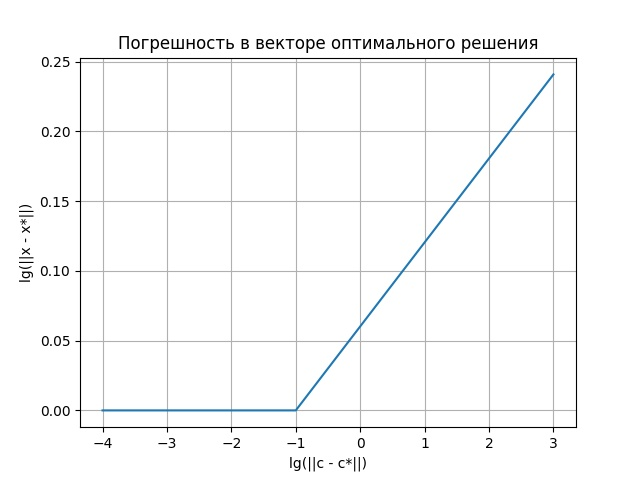
\includegraphics[scale=0.85]{Graphic 1.jpg}}
\label{fig:image}
\end{figure}

\begin{figure}[H]
\center{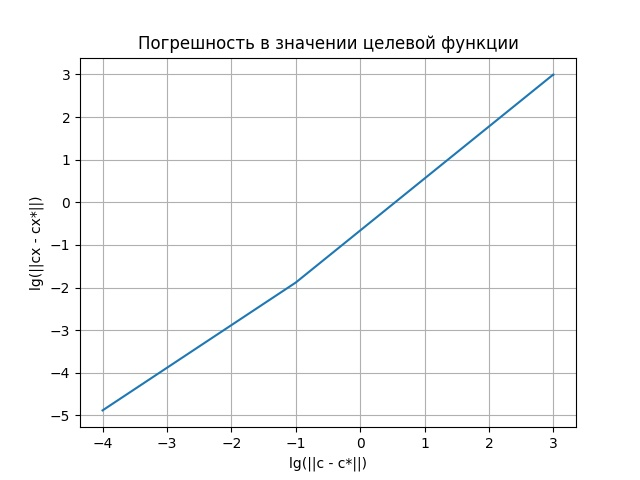
\includegraphics[scale=0.85]{Graphic 2.jpg}}
\label{fig:image}
\end{figure}


\noindent \paragraph{Анализ полученных графиков} 
\label{gr}
\\\\
В общем виде целевая функция задачи линейного программирования записывается следующим образом: $F=c_1x_1 + c_2x_2 + c_3x_3 + c_4x_4 + c_5x_5$.\\
Оптимальной точкой задачи будет являться та, в которой гиперплоскость $F$ касается множества допустимых точек. Изменение значений коэффициентов $c_1, c_2, c_3, c_4, c_5$ приводит к изменению угла наклона гиперплоскости $F$. Графическая интерпретация даёт нам понять, что это может привести к изменению оптимального решения: оно будет достигаться в другой вершине пространства решений. Однако, при небольших изменениях в коэффициентах функции цели, оптимальная вершина не меняется.

\section{Программная реализация}
\noindent В процессе реализации алгоритмов использовался язык программирования Python3.6. Для построения графиков и  проверки полученных решений пользовались пакетом MATLAB2020b.
\\\\
\noindent Исходный код находится в системе контроля версий GitHub 
\\
URL: https://github.com/Brightest-Sunshine/Optimization-methods-2021/tree/master/lab1/code

\section{Выводы}
\noindent Симплекс-метод эффективен на практике. Вычислительная эффективность оценивается обычно при помощи двух параметров:
\begin{enumerate}
    \item числа итераций, необходимого для получения решения
    \item затрат машинного времени
\end{enumerate}
\\\\
\noindent В результате численных экспериментов произведенных в 1972 году Кли и Минти были полученые следующие результаты:
\begin{enumerate}
    \item Число итераций при решении задач линейного программирования в стандартной форме с $m$ ограничениями и n переменными заключено между $m$ и $3m$
    \item Среднее число итераций $2m$. Верхняя граница числа итераций равна $2m+n$
    \item Требуемое машинное время пропорционально $m^3$
    \item Число ограничений больше влияет на вычислительную эффективность, чем число переменных, поэтому при формулировке задач линейного программирования нужно стремиться к уменьшению числа ограничений пусть даже путём роста числа переменных
\end{enumerate}

\section{Дополнительные пояснения на замечания}
В ходе защиты данной лабораторной работы, преподавателем были выявлены замечания. Ниже приведены ссылки, которые переместят в ту часть отчета, которая была отредактирована.
\begin{itemize}
    \item Показана справедливость теоремы о связи решений прямой и двойственной задач \eqref{show}.
   \item Более подробно расписана оценка достоверности полученного результата \eqref{mark}.
   \item Были добавлены более подробные комментарии к полученным зависимостям погрешности в значении целевой функции и векторе оптимального решения \eqref{gr}.
   \item В качестве отдельного пункта в отчет были вынесены результаты работы программной реализации симплекс-метода вместе с входными данными, использованными для построения решения \eqref{res}.
\end{itemize}
   
\section{Результаты работы программы}
\label{res}
\noindent В результате тестирования программной реализации симплекс-метода была проверена обозначенная в отчете задача и получены следующие результаты:

\begin{figure}[H]
\center{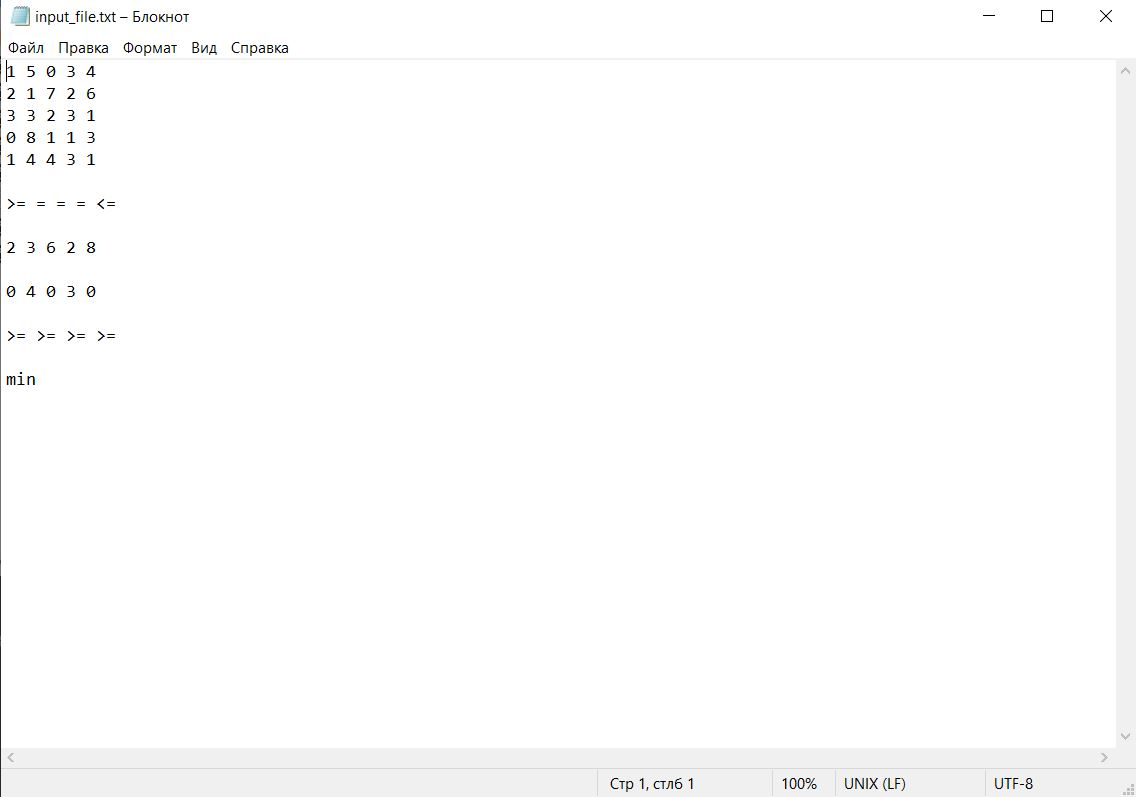
\includegraphics[scale=0.75]{Input_data.JPG}}
\label{fig:image}
\end{figure}

\begin{figure}[H]
\center{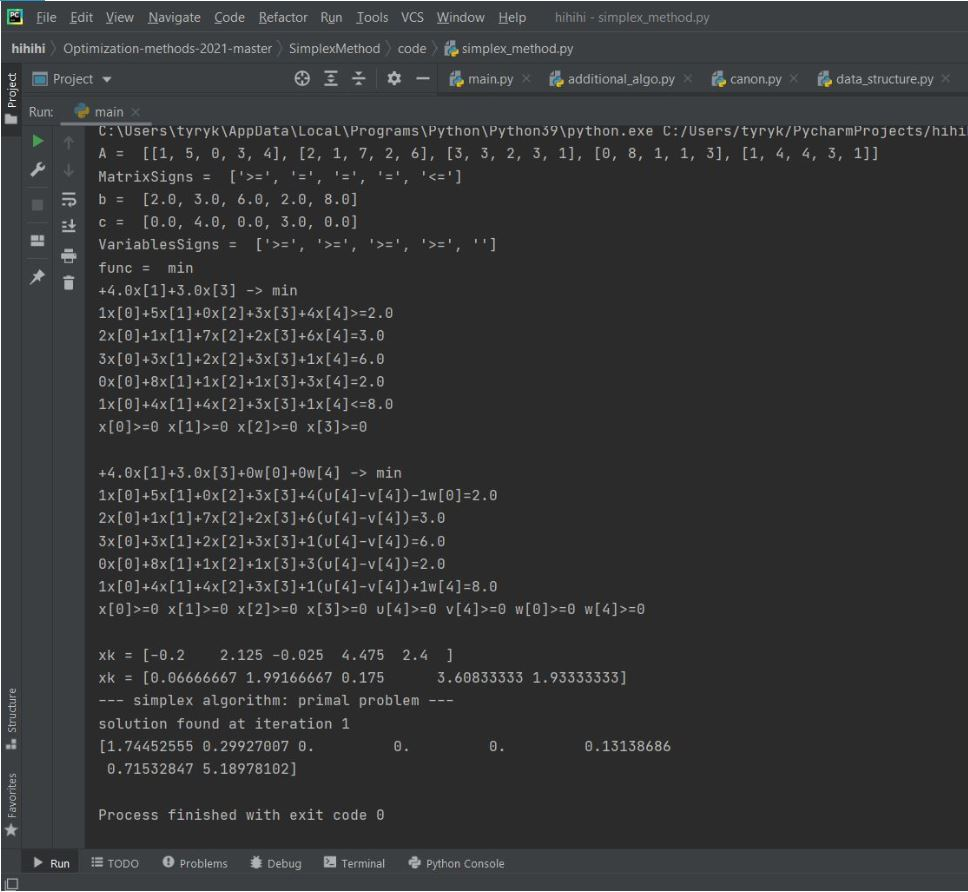
\includegraphics[scale=0.75]{out.JPG}}
\label{fig:image}
\end{figure}

	\begin{thebibliography}{99}
		\bibitem{petuh} Петухов Л. В. Методы оптимизации. Задачи выпуклого программирования: учеб. пособие / Л. В. Петухов, Г. А. Серёгин, Е. А. Родионова. -- СПб.: Изд-во Политехн. ун-та, 2014. -- 99 с.
		\bibitem{akulich} Акулич И.Л. Математическое программирование в примерах и задачах: учеб. пособие. -- СПб.: Изд-во 'Лань', 2011. -- 352с.: ил.
	\end{thebibliography}
	
\end{document}
